\documentclass[a4paper,11pt,titlepage]{article}
% The maths package
\usepackage{amsmath}
% The graphics package
\usepackage{graphicx}
% Allows paragraph in blocks
\usepackage{parskip}
% Code hightling
\usepackage{minted}
% Verbatim file inclusion
\usepackage{fancyvrb}

%%%%%%%%%%%%%%%%%%%%%%%%%%%%%%%% Define the title %%%%%%%%%%%%%%%%%%%%%%%%%%%%%%
\title{
MECH3750 Engineering Analysis II \\ 
Assignment 1: Buckling analysis
}
% define the author
\author{
Merrick Heley\\
42339915
\and
Sophia Impiccini\\
42650852
}

%%%%%%%%%%%%%%%%%%%%%%%%%%%%%% Notes and commands %%%%%%%%%%%%%%%%%%%%%%%%%%%%%%
% \section*{Task 1} uses an asterisk to suppress the section number

% This command adds \ud for finishing integrals
\newcommand{\ud}{\,\mathrm{d}}

% Set the pygmentation style for code
% pygmentize -L styles
\usemintedstyle{autumn}

% Simple command for python file input
\newcommand{\inputpython}[1]{
    \inputminted[linenos=true, 
                 frame=single, 
                 fontsize=\scriptsize, 
                 label=#1]
                {python}{#1}
}

% Simple command for python file output
\newcommand{\pythonoutput}[1]{
    \immediate\write18{python #1 > #1.out}
    \fvset{frame=single, numbers=left, fontsize=\scriptsize, label=#1.out}
    \VerbatimInput{#1.out}
    \write18{del #1.out}
}

%%%%%%%%%%%%%%%%%%%%%%%%%%%%%%%% Start document %%%%%%%%%%%%%%%%%%%%%%%%%%%%%%%%

\begin{document}
% generates the title
\maketitle

%%%%%%%%%%%%%%%%%%%%%%%%%%%%%%%%%% TASK 1 %%%%%%%%%%%%%%%%%%%%%%%%%%%%%%%%%%%%%%
\section*{Task 1}

The Euler load is the load where the spring initially begins to bend.

\begin{figure}[!hbp]
\centering
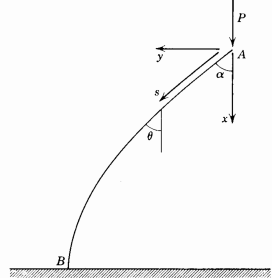
\includegraphics{buckling.png}
\caption{Buckling example}
\end{figure}

Where P is the load at A, $\theta$ is the angle of the bend at distance s 
from A.

For a rod placed vertically and fixed at end B, it can be seen that the initial
value of $\alpha$ is 0$^\circ$.

Using the given equation

\begin{equation}
L = 
\sqrt{\frac{EI}{P}} 
\int_0^{\frac{\pi}{2}} 
    {\displaystyle{\left[
        1-\sin^2{\left(\frac{\alpha}{2}\right)}\sin^2{\phi}
    \right]^{1/2}}}
\ud \phi
\end{equation}

and substituting in the observation that the Euler load will be applied when the
rod is vertical

\begin{equation}
\alpha = 0 \text{ when } P = P_e
\end{equation}
the equation can be simplified 
n
\begin{align}
L & = 
\sqrt{\frac{EI}{P_e}} 
\int_0^{\frac{\pi}{2}} 
    {\displaystyle{\left[
        1-\sin^2{\left(\frac{0}{2}\right)}\sin^2{\phi}
    \right]^{1/2}}}
\ud \phi \notag\\
& = 
\sqrt{\frac{EI}{P_e}} 
\int_0^{\frac{\pi}{2}} 
    {\displaystyle{\left[
        1-\sin^2{0}\sin^2{\phi}
    \right]^{1/2}}}
\ud \phi \notag\\
& = 
\sqrt{\frac{EI}{P_e}} 
\int_0^{\frac{\pi}{2}} 
    {\displaystyle{\left[
        1
    \right]^{1/2}}}
\ud \phi \notag\\
& = 
\sqrt{\frac{EI}{P_e}} 
\int_0^{\frac{\pi}{2}} \ud \phi \notag\\
& = \sqrt{\frac{EI}{P_e}} \left(\frac{\pi}{2} - 0\right) \notag\\
& = \frac{\pi}{2} \sqrt{\frac{EI}{P_e}} \notag\\
\intertext{and rearranged for $P_e$} \notag\\
\frac{2L}{\pi} & = \sqrt{\frac{EI}{P_e}} \notag\\ 
\frac{4L^2}{\pi^2} & = \frac{EI}{P_e} \notag\\
P_e & = \frac{\pi^2 EI}{4L^2}
\end{align}
\clearpage

%%%%%%%%%%%%%%%%%%%%%%%%%%%%%%%%%% TASK 2 %%%%%%%%%%%%%%%%%%%%%%%%%%%%%%%%%%%%%%
\section*{Task 2}
The code below implements an adaptive integrator that may take Gaussian
quadrature functions as input.

The ouput of the adaptive integrator test is provided, showing how closely the
integrator matches the SciPy integrator.
\inputpython{integrator.py}
\pythonoutput{integrator.py}

It can be seen from the output that the adaptive integrator is quite accurate
compared to the module provided by SciPy.
\clearpage

%%%%%%%%%%%%%%%%%%%%%%%%%%%%%%%%%% TASK 3 %%%%%%%%%%%%%%%%%%%%%%%%%%%%%%%%%%%%%%
\section*{Task 3}
\clearpage
\end{document}